\section{Robert Jacak}
\label{sec:RobertJacak}

\subsection{Zdjecie}
\centering Poniżej widzimy zdjęcie zebry
\begin{figure}[htbt]
    \centering
    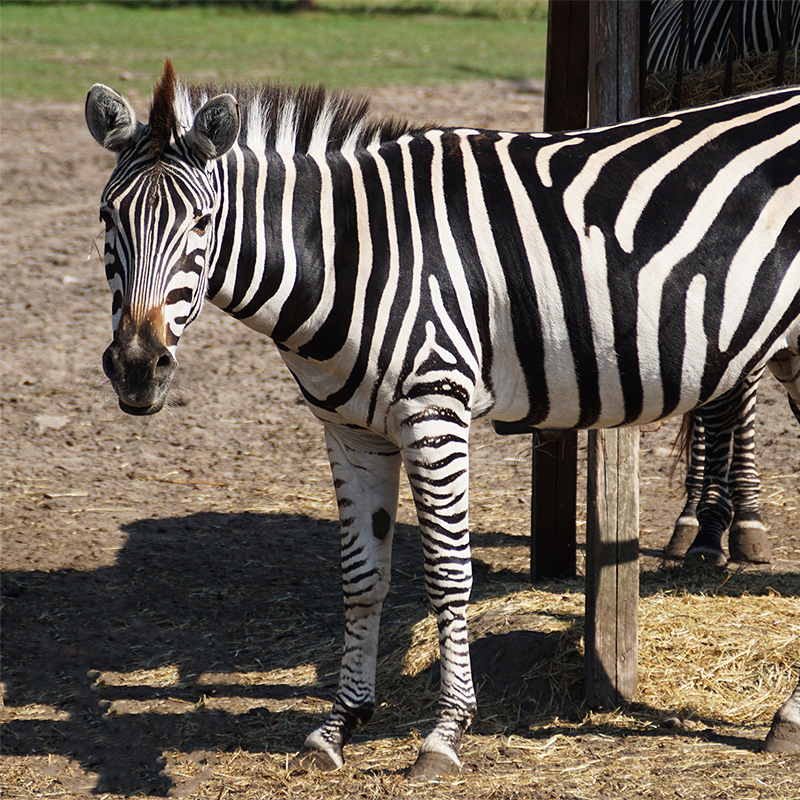
\includegraphics [scale=0.3]{pictures/zebra.jpg}
    \caption{Zebra bobo}
    \label{fig:zebra}
\end{figure}
\subsection{5 najlepszych miejsc, żeby zobaczyć zebre}
\begin{enumerate}
    \item SERENGETI NATIONAL PARK, TANZANIA
    \item MAKGADIKGADI PANS, BOTSWANA
    \item ETOSHA NATIONAL PARK, NAMIBIA
    \item LEWA CONSERVANCY, KENYA
    \item KLEIN KAROO, SOUTH AFRICA
\end{enumerate}
\subsection{Gatunki zebry}
\begin{itemize}
    \item [!!!] zebra flamingowa
    \item [..] zebra stepowa
    \item [O] zebra równikowa
    \item zebra sawannowa
    
\end{itemize}
\subsection{Ceny biletow w zoo we Wrocławiu}
\begin{tabular}{lccc}
\multicolumn{4}{c}{\textbf{Bilety indywidualne}}                                                      \\
\multicolumn{1}{c}{}             & Ceny standardowe & Ceny zoo na ratunek & Ceny dla posiadaczy karty \\
\multicolumn{1}{c}{Bilet ulgowy} & 60 zl            & 61 zl               & 20 zl                     \\
Bilet normalny                   & 70 zl            & 71 zl               & 30 zl                     \\
Bilet studencki                  & 65 zl            & 66 zl               &                           \\
Bilet rodzinny                   & 230 zl           & 235 zl              & 145 zl                   
\end{tabular}
\label{tab:Ceny}
\subsection{Prawo de Morgana}
\begin{equation}
    \left ( \sim \left ( p \wedge q \right ) \right ) \Leftrightarrow \left ( \left ( \sim p \right ) \vee \left ( \sim q \right ) \right )
\end{equation}
\subsection{Tekst}
    Moim zdaniem to nie ma tak, że dobrze albo że nie dobrze. Gdybym miał powiedzieć, co cenię w życiu najbardziej, powiedziałbym, że \textbf{ludzi}. Ekhm... Ludzi, którzy podali mi pomocną dłoń, kiedy sobie nie radziłem, kiedy byłem sam. I co ciekawe, to właśnie przypadkowe spotkania wpływają na nasze życie. Chodzi o to, że kiedy wyznaje się pewne wartości, nawet pozornie uniwersalne, bywa, że nie znajduje się zrozumienia, które by tak rzec, które pomaga się nam rozwijać. Ja miałem szczęście, by tak rzec, ponieważ je znalazłem. I dziękuję życiu. Dziękuję mu, \textbf{życie to śpiew, życie to taniec, życie to miłość}. Wielu ludzi pyta mnie o to samo, ale jak ty to robisz?, skąd czerpiesz tę radość? A ja odpowiadam, że to proste, to \underline {umiłowanie życia}, to właśnie ono sprawia, że dzisiaj na przykład buduję maszyny, a jutro... kto wie, dlaczego by nie, oddam się pracy społecznej i będę ot, choćby sadzić... znaczy... marchew.
\subsection{Odwołania}
 Jedyne co trzeba zrobić, żeby zobaczyć tą \ref{fig:zebra} zebrę to kupić bilet do zoo we Wrocławiu \ref{tab:Ceny}